% Options for packages loaded elsewhere
\PassOptionsToPackage{unicode}{hyperref}
\PassOptionsToPackage{hyphens}{url}
%
\documentclass[
]{article}
\usepackage{lmodern}
\usepackage{amssymb,amsmath}
\usepackage{ifxetex,ifluatex}
\ifnum 0\ifxetex 1\fi\ifluatex 1\fi=0 % if pdftex
  \usepackage[T1]{fontenc}
  \usepackage[utf8]{inputenc}
  \usepackage{textcomp} % provide euro and other symbols
\else % if luatex or xetex
  \usepackage{unicode-math}
  \defaultfontfeatures{Scale=MatchLowercase}
  \defaultfontfeatures[\rmfamily]{Ligatures=TeX,Scale=1}
\fi
% Use upquote if available, for straight quotes in verbatim environments
\IfFileExists{upquote.sty}{\usepackage{upquote}}{}
\IfFileExists{microtype.sty}{% use microtype if available
  \usepackage[]{microtype}
  \UseMicrotypeSet[protrusion]{basicmath} % disable protrusion for tt fonts
}{}
\makeatletter
\@ifundefined{KOMAClassName}{% if non-KOMA class
  \IfFileExists{parskip.sty}{%
    \usepackage{parskip}
  }{% else
    \setlength{\parindent}{0pt}
    \setlength{\parskip}{6pt plus 2pt minus 1pt}}
}{% if KOMA class
  \KOMAoptions{parskip=half}}
\makeatother
\usepackage{xcolor}
\IfFileExists{xurl.sty}{\usepackage{xurl}}{} % add URL line breaks if available
\IfFileExists{bookmark.sty}{\usepackage{bookmark}}{\usepackage{hyperref}}
\hypersetup{
  pdftitle={Shiny Application for Genetic Management of Colonies},
  pdfauthor={R. Mark Sharp},
  hidelinks,
  pdfcreator={LaTeX via pandoc}}
\urlstyle{same} % disable monospaced font for URLs
\usepackage[margin=1in]{geometry}
\usepackage{color}
\usepackage{fancyvrb}
\newcommand{\VerbBar}{|}
\newcommand{\VERB}{\Verb[commandchars=\\\{\}]}
\DefineVerbatimEnvironment{Highlighting}{Verbatim}{commandchars=\\\{\}}
% Add ',fontsize=\small' for more characters per line
\usepackage{framed}
\definecolor{shadecolor}{RGB}{248,248,248}
\newenvironment{Shaded}{\begin{snugshade}}{\end{snugshade}}
\newcommand{\AlertTok}[1]{\textcolor[rgb]{0.94,0.16,0.16}{#1}}
\newcommand{\AnnotationTok}[1]{\textcolor[rgb]{0.56,0.35,0.01}{\textbf{\textit{#1}}}}
\newcommand{\AttributeTok}[1]{\textcolor[rgb]{0.77,0.63,0.00}{#1}}
\newcommand{\BaseNTok}[1]{\textcolor[rgb]{0.00,0.00,0.81}{#1}}
\newcommand{\BuiltInTok}[1]{#1}
\newcommand{\CharTok}[1]{\textcolor[rgb]{0.31,0.60,0.02}{#1}}
\newcommand{\CommentTok}[1]{\textcolor[rgb]{0.56,0.35,0.01}{\textit{#1}}}
\newcommand{\CommentVarTok}[1]{\textcolor[rgb]{0.56,0.35,0.01}{\textbf{\textit{#1}}}}
\newcommand{\ConstantTok}[1]{\textcolor[rgb]{0.00,0.00,0.00}{#1}}
\newcommand{\ControlFlowTok}[1]{\textcolor[rgb]{0.13,0.29,0.53}{\textbf{#1}}}
\newcommand{\DataTypeTok}[1]{\textcolor[rgb]{0.13,0.29,0.53}{#1}}
\newcommand{\DecValTok}[1]{\textcolor[rgb]{0.00,0.00,0.81}{#1}}
\newcommand{\DocumentationTok}[1]{\textcolor[rgb]{0.56,0.35,0.01}{\textbf{\textit{#1}}}}
\newcommand{\ErrorTok}[1]{\textcolor[rgb]{0.64,0.00,0.00}{\textbf{#1}}}
\newcommand{\ExtensionTok}[1]{#1}
\newcommand{\FloatTok}[1]{\textcolor[rgb]{0.00,0.00,0.81}{#1}}
\newcommand{\FunctionTok}[1]{\textcolor[rgb]{0.00,0.00,0.00}{#1}}
\newcommand{\ImportTok}[1]{#1}
\newcommand{\InformationTok}[1]{\textcolor[rgb]{0.56,0.35,0.01}{\textbf{\textit{#1}}}}
\newcommand{\KeywordTok}[1]{\textcolor[rgb]{0.13,0.29,0.53}{\textbf{#1}}}
\newcommand{\NormalTok}[1]{#1}
\newcommand{\OperatorTok}[1]{\textcolor[rgb]{0.81,0.36,0.00}{\textbf{#1}}}
\newcommand{\OtherTok}[1]{\textcolor[rgb]{0.56,0.35,0.01}{#1}}
\newcommand{\PreprocessorTok}[1]{\textcolor[rgb]{0.56,0.35,0.01}{\textit{#1}}}
\newcommand{\RegionMarkerTok}[1]{#1}
\newcommand{\SpecialCharTok}[1]{\textcolor[rgb]{0.00,0.00,0.00}{#1}}
\newcommand{\SpecialStringTok}[1]{\textcolor[rgb]{0.31,0.60,0.02}{#1}}
\newcommand{\StringTok}[1]{\textcolor[rgb]{0.31,0.60,0.02}{#1}}
\newcommand{\VariableTok}[1]{\textcolor[rgb]{0.00,0.00,0.00}{#1}}
\newcommand{\VerbatimStringTok}[1]{\textcolor[rgb]{0.31,0.60,0.02}{#1}}
\newcommand{\WarningTok}[1]{\textcolor[rgb]{0.56,0.35,0.01}{\textbf{\textit{#1}}}}
\usepackage{longtable,booktabs}
% Correct order of tables after \paragraph or \subparagraph
\usepackage{etoolbox}
\makeatletter
\patchcmd\longtable{\par}{\if@noskipsec\mbox{}\fi\par}{}{}
\makeatother
% Allow footnotes in longtable head/foot
\IfFileExists{footnotehyper.sty}{\usepackage{footnotehyper}}{\usepackage{footnote}}
\makesavenoteenv{longtable}
\usepackage{graphicx,grffile}
\makeatletter
\def\maxwidth{\ifdim\Gin@nat@width>\linewidth\linewidth\else\Gin@nat@width\fi}
\def\maxheight{\ifdim\Gin@nat@height>\textheight\textheight\else\Gin@nat@height\fi}
\makeatother
% Scale images if necessary, so that they will not overflow the page
% margins by default, and it is still possible to overwrite the defaults
% using explicit options in \includegraphics[width, height, ...]{}
\setkeys{Gin}{width=\maxwidth,height=\maxheight,keepaspectratio}
% Set default figure placement to htbp
\makeatletter
\def\fps@figure{htbp}
\makeatother
\setlength{\emergencystretch}{3em} % prevent overfull lines
\providecommand{\tightlist}{%
  \setlength{\itemsep}{0pt}\setlength{\parskip}{0pt}}
\setcounter{secnumdepth}{-\maxdimen} % remove section numbering

\title{Shiny Application for Genetic Management of Colonies}
\author{R. Mark Sharp}
\date{}

\begin{document}
\maketitle

\hypertarget{introduction}{%
\subsection{Introduction}\label{introduction}}

This tutorial demonstrates the major functions used within the Shiny
application provided by the \textbf{nprcmanager} package. This is a
brief tutorial that illustrates a typical workflow and does not explore
all possible workflows.

Please provide any comments, questions, or bug reports through the
GitHub issue tracker at
\url{https://github.com/rmsharp/nprcmanager/issues}.

\hypertarget{installation-and-help}{%
\subsection{Installation and Help}\label{installation-and-help}}

To get the most recent version you can install \textbf{nprcmanager} from
GitHub with the following code.

\begin{Shaded}
\begin{Highlighting}[]
\KeywordTok{install.packages}\NormalTok{(}\StringTok{"devtools"}\NormalTok{)}
\NormalTok{devtools}\OperatorTok{::}\KeywordTok{install_github}\NormalTok{(}\StringTok{"rmsharp/nprcmanager"}\NormalTok{)}
\end{Highlighting}
\end{Shaded}

All missing dependencies should be automatically installed.

You can start the Shiny application from the \textbf{R} console with

\begin{Shaded}
\begin{Highlighting}[]
\KeywordTok{library}\NormalTok{(nprcmanager)}
\CommentTok{#runManager()}
\KeywordTok{getwd}\NormalTok{()}
\end{Highlighting}
\end{Shaded}

This will result in the opening screen where you tell the application
how to find the pedigree you will be using.

\hypertarget{input}{%
\subsection{Input}\label{input}}

\hypertarget{pedigree-file-structure}{%
\subsubsection{Pedigree File Structure}\label{pedigree-file-structure}}

Most of the screen is filled with information about formatting a text or
Excel worksheet pedigree file.

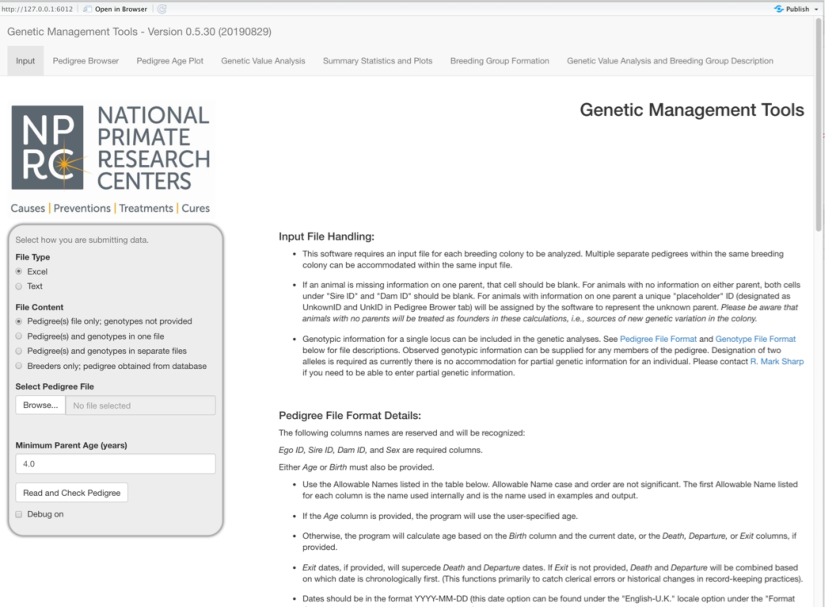
\includegraphics{shiny_app_use_files/figure-latex/eopening-screen-top-1.pdf}

\begin{center}\rule{0.5\linewidth}{\linethickness}\end{center}

Scrolling down to the middle of the opening screen exposes a table that
describes a pedigree file and further instructions.

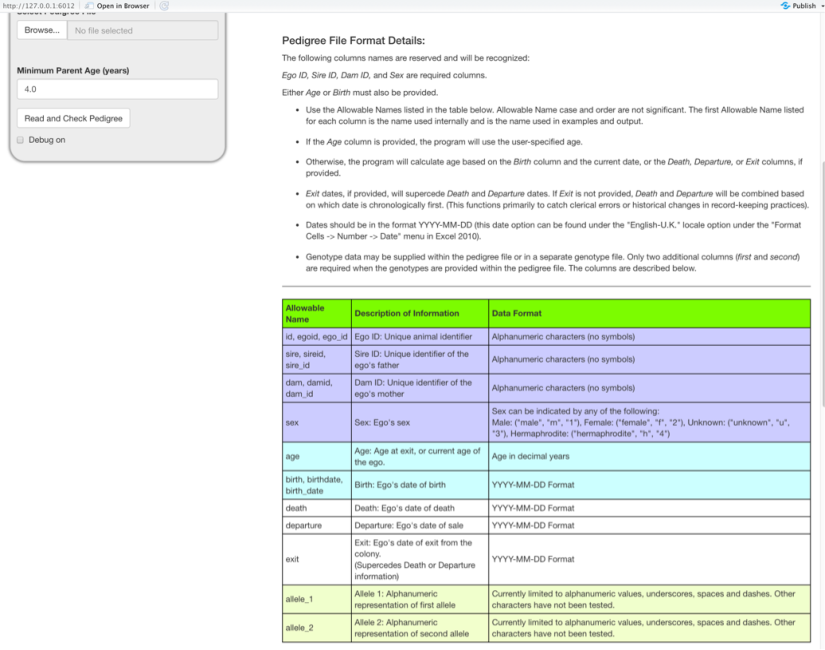
\includegraphics{shiny_app_use_files/figure-latex/eopening-screen-middle-1.pdf}

\begin{center}\rule{0.5\linewidth}{\linethickness}\end{center}

Scrolling down to the bottom of the opening screen exposes more pedigree
file instructions, a table that describes a genotype file and
instructions regarding use of a genotype file. This tutorial will not
include instructions on using a genotype file.

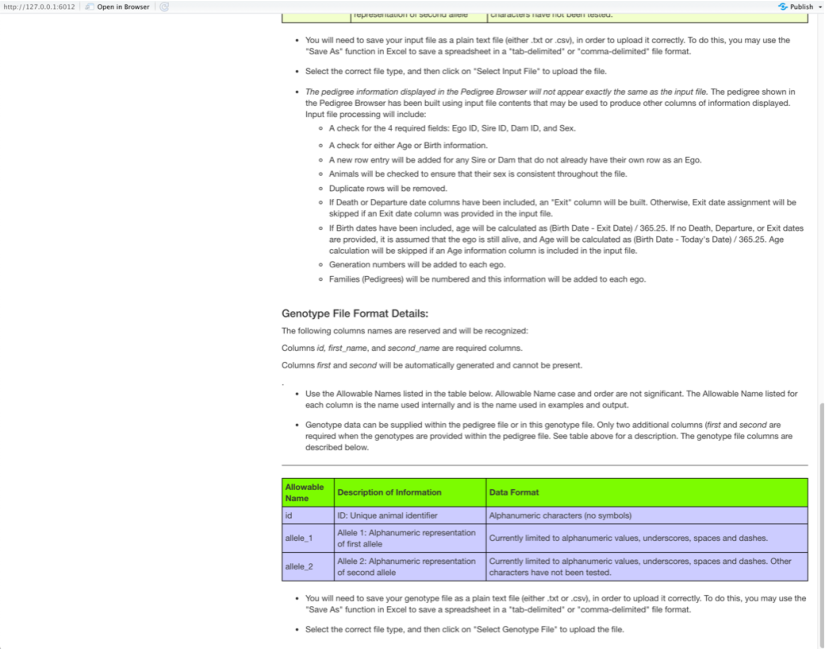
\includegraphics{shiny_app_use_files/figure-latex/eopening-screen-bottom-1.pdf}

\begin{center}\rule{0.5\linewidth}{\linethickness}\end{center}

\hypertarget{reading-in-the-pedigree}{%
\subsubsection{Reading in the Pedigree}\label{reading-in-the-pedigree}}

In this introductory tutorial, we will use an Excel file containing a
hypothetical pedigree of macaques. We will work with the gray box on the
left at the top of the screen.

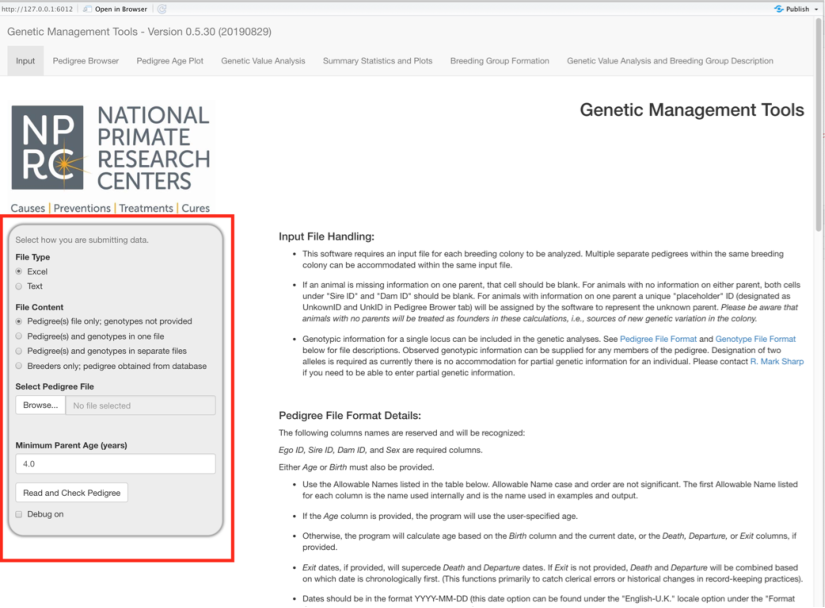
\includegraphics{shiny_app_use_files/figure-latex/eopening-screen-top-red-oval-1.pdf}

\begin{center}\rule{0.5\linewidth}{\linethickness}\end{center}

A Microsoft Excel workbook with a single worksheet is the default file
type; though comma (.csv), semi-colon (.txt), and tab (.txt) separated
value files are all acceptable formats.

The \emph{Example\_Pedigree.xlsx} file we are using is from a CSV file
created as shown below and then saved in an Excel format.

\begin{Shaded}
\begin{Highlighting}[]
\KeywordTok{makeExamplePedigreeFile}\NormalTok{()}
\end{Highlighting}
\end{Shaded}

Select the \textbf{Browse} button and select the pedigree file from your
file system.

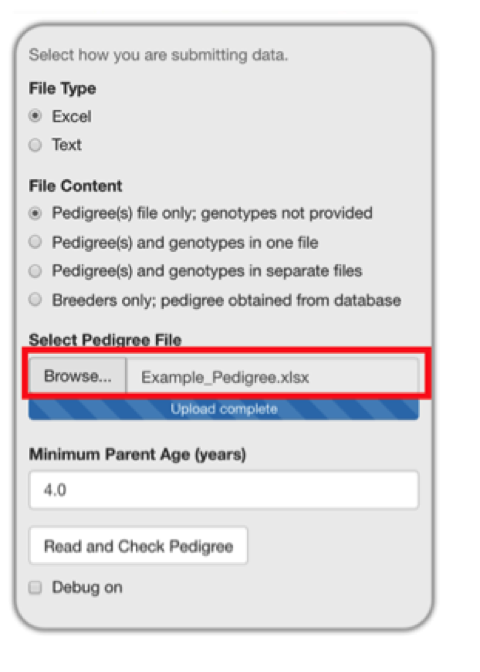
\includegraphics{shiny_app_use_files/figure-latex/example-pedigree-1.pdf}

\begin{center}\rule{0.5\linewidth}{\linethickness}\end{center}

It is important to make sure the minimum parent age is low enough for
the animals in your pedigree. For our example pedigree, we are changing
it from 4 years to 2 years of age since these macaques may reproduce as
early as two years of age. This is shown below in three progressive
images with the center image demonstrating how the hovertext provides an
explanation of how this value is used.

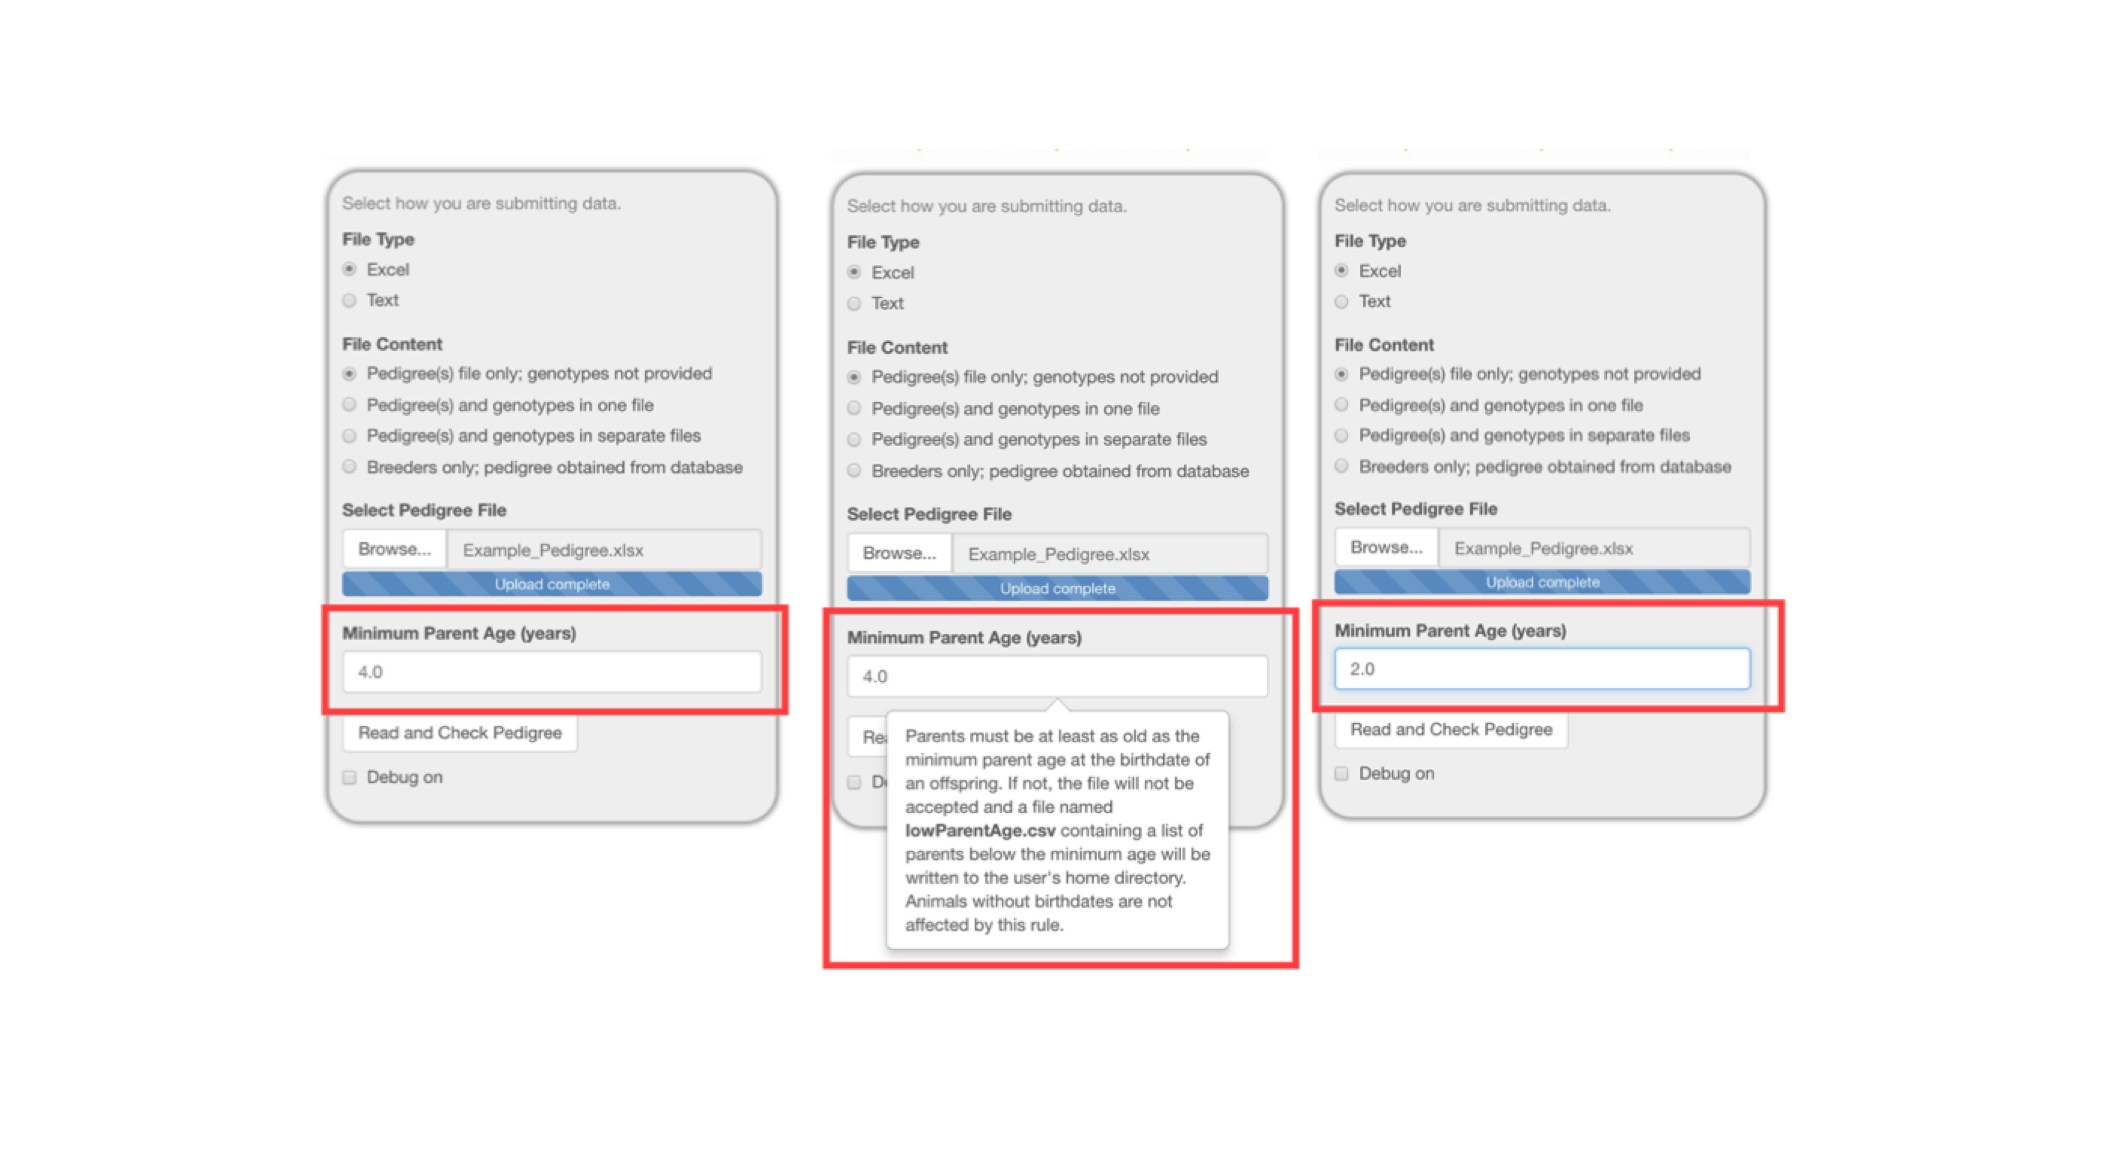
\includegraphics{shiny_app_use_files/figure-latex/example-pedigree-minParentAgeSequence-1.pdf}

\begin{center}\rule{0.5\linewidth}{\linethickness}\end{center}

\hypertarget{reading-in-a-pedigree-and-testing-for-errors}{%
\subsubsection{Reading in a Pedigree and Testing for
Errors}\label{reading-in-a-pedigree-and-testing-for-errors}}

Selected \textbf{Read and Check Pedigree} will read in the file and test
to see if the pedigree file has all of the columns needed and the
pedigree is internally consistent.

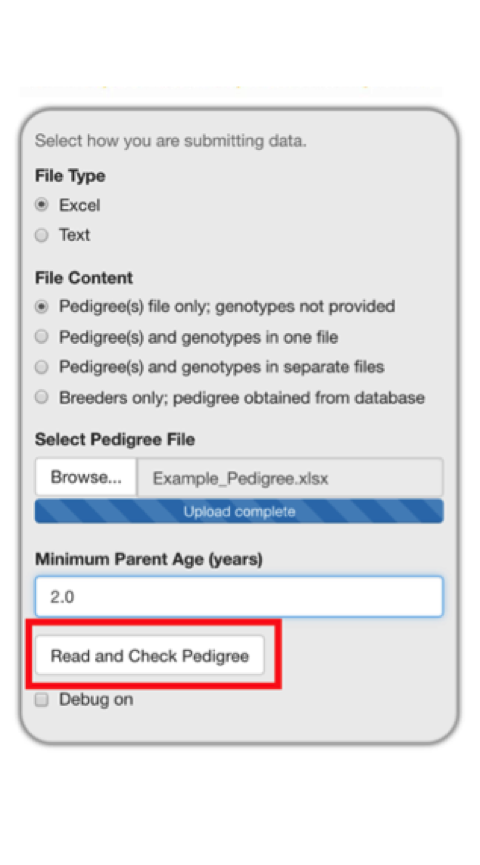
\includegraphics{shiny_app_use_files/figure-latex/read-and-check-pedigree-1.pdf}

\begin{center}\rule{0.5\linewidth}{\linethickness}\end{center}

Several error types, shown below, are detected the application.

\begin{longtable}[]{@{}ll@{}}
\toprule
Error & Definition\tabularnewline
\midrule
\endhead
failedDatabaseConnection & Database connection failed: configuration or
permissions are invalid\tabularnewline
missingColumns & Columns that must be within the pedigree file are
missing.\tabularnewline
invalidDateRows & Values, which are supposed to be dates, cannot be
interpreted as a date.\tabularnewline
suspiciousParents & Parents were too young on the date of birth of to
have been the parent.\tabularnewline
femaleSires & Individuals listed as female or hermaphroditic and as a
sire.\tabularnewline
maleDams & Individuals are listed as male and as a dam.\tabularnewline
sireAndDam & Individuals who are listed as both a sire and a
dam.\tabularnewline
duplicateIds & IDs listed more than once.\tabularnewline
fatalError & Fatal Errors.\tabularnewline
changedCols & Columns that have been changed to conform to internal
naming conventions and what they were changed to.\tabularnewline
\bottomrule
\end{longtable}

\begin{center}\rule{0.5\linewidth}{\linethickness}\end{center}

\hypertarget{pedigree-browser}{%
\subsection{Pedigree Browser}\label{pedigree-browser}}

The \textbf{Pedigree Browser} tab defaults to displaying 10 rows of the
pedigree at a time, but you can choose to display 10, 25, 50, or 100
rows. You can choose to display UNKNOWN IDs in the rows displayed.

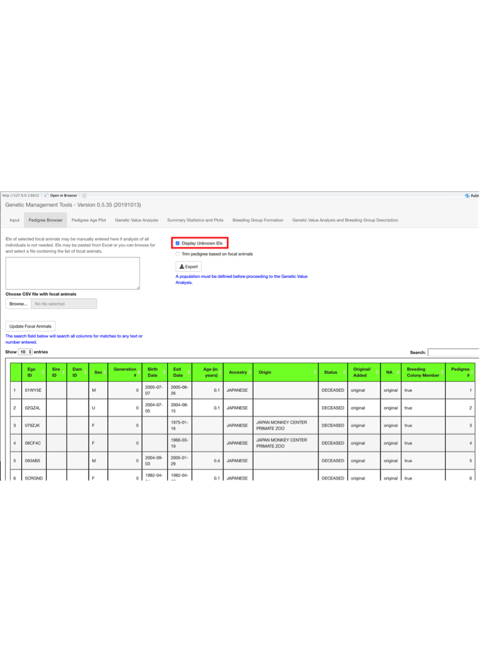
\includegraphics{shiny_app_use_files/figure-latex/pb-100-rows-display-unknown-ids-1.pdf}

\begin{center}\rule{0.5\linewidth}{\linethickness}\end{center}

\hypertarget{a-note-about-obfuscated-data}{%
\subsubsection{A Note About Obfuscated
Data}\label{a-note-about-obfuscated-data}}

I have place red lines under the UNKNOWN IDs in the partial pedigree
list below for clarity. These IDs have no meaning other than they all
begin with the letter \emph{U} and are following with a left
alphanumeric string of five places. The form of this ID is set by the
\emph{obfuscateId} function.

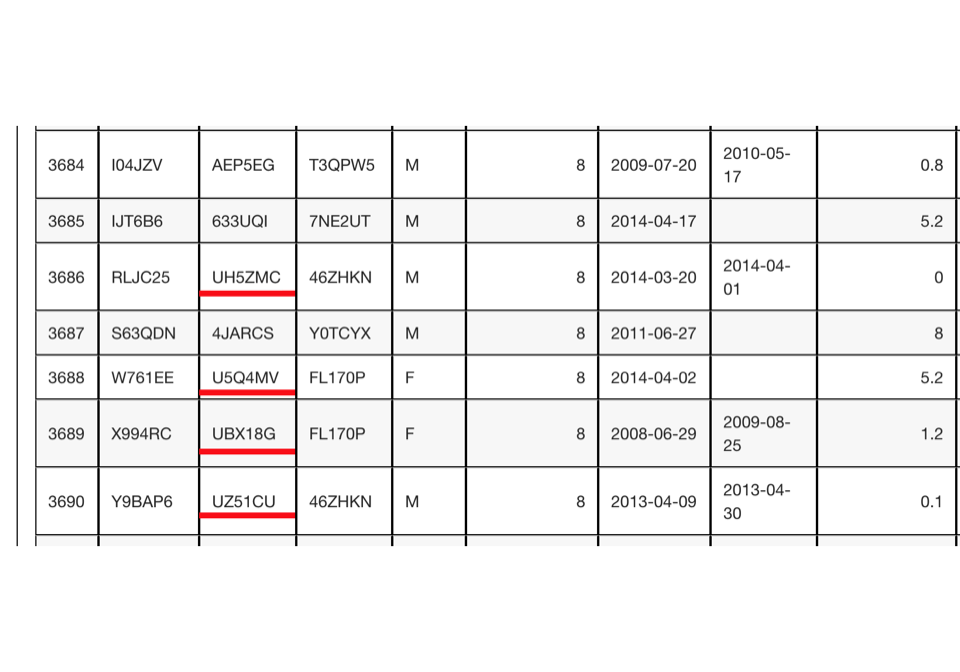
\includegraphics{shiny_app_use_files/figure-latex/unknown-displayed-1.pdf}

\begin{center}\rule{0.5\linewidth}{\linethickness}\end{center}

\hypertarget{unknown-ids}{%
\subsubsection{Unknown IDs}\label{unknown-ids}}

In this example pedigree, when you deselect the \textbf{Display Unknown
IDs} checkbox. The number of rows reduces from 3,694 to 2,322, because
there were 1,372 UNKNOWN animals generated when constructing the
pedigree to provide sire and dam placeholders for all animals.

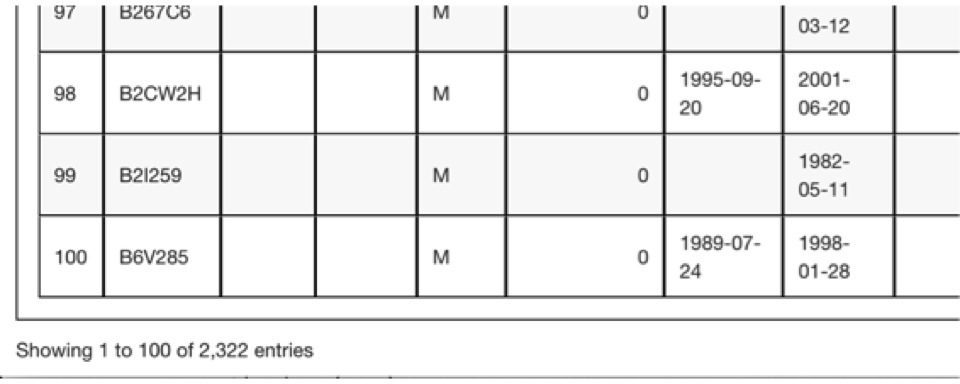
\includegraphics{shiny_app_use_files/figure-latex/no-unknown-displayed-1.pdf}

\begin{center}\rule{0.5\linewidth}{\linethickness}\end{center}

\hypertarget{selecting-a-pedigree-subset-focal-animals}{%
\subsubsection{Selecting a Pedigree Subset --- Focal
Animals}\label{selecting-a-pedigree-subset-focal-animals}}

The \textbf{Pedigree Browser} tab displays the full pedigree by default
but allows you to select a subset of the pedigree by entering a list of
animals of interest (\emph{focal animals}).

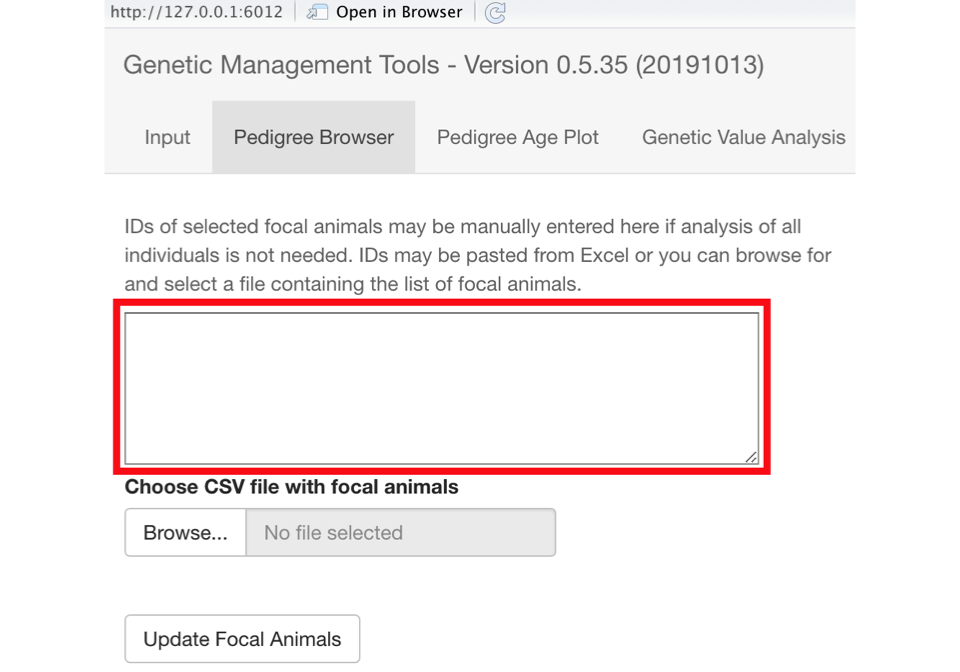
\includegraphics{shiny_app_use_files/figure-latex/focal-animal-text-box-1.pdf}

\begin{center}\rule{0.5\linewidth}{\linethickness}\end{center}

You can enter in the animal IDs by typing them into the text box
directly as shown below.

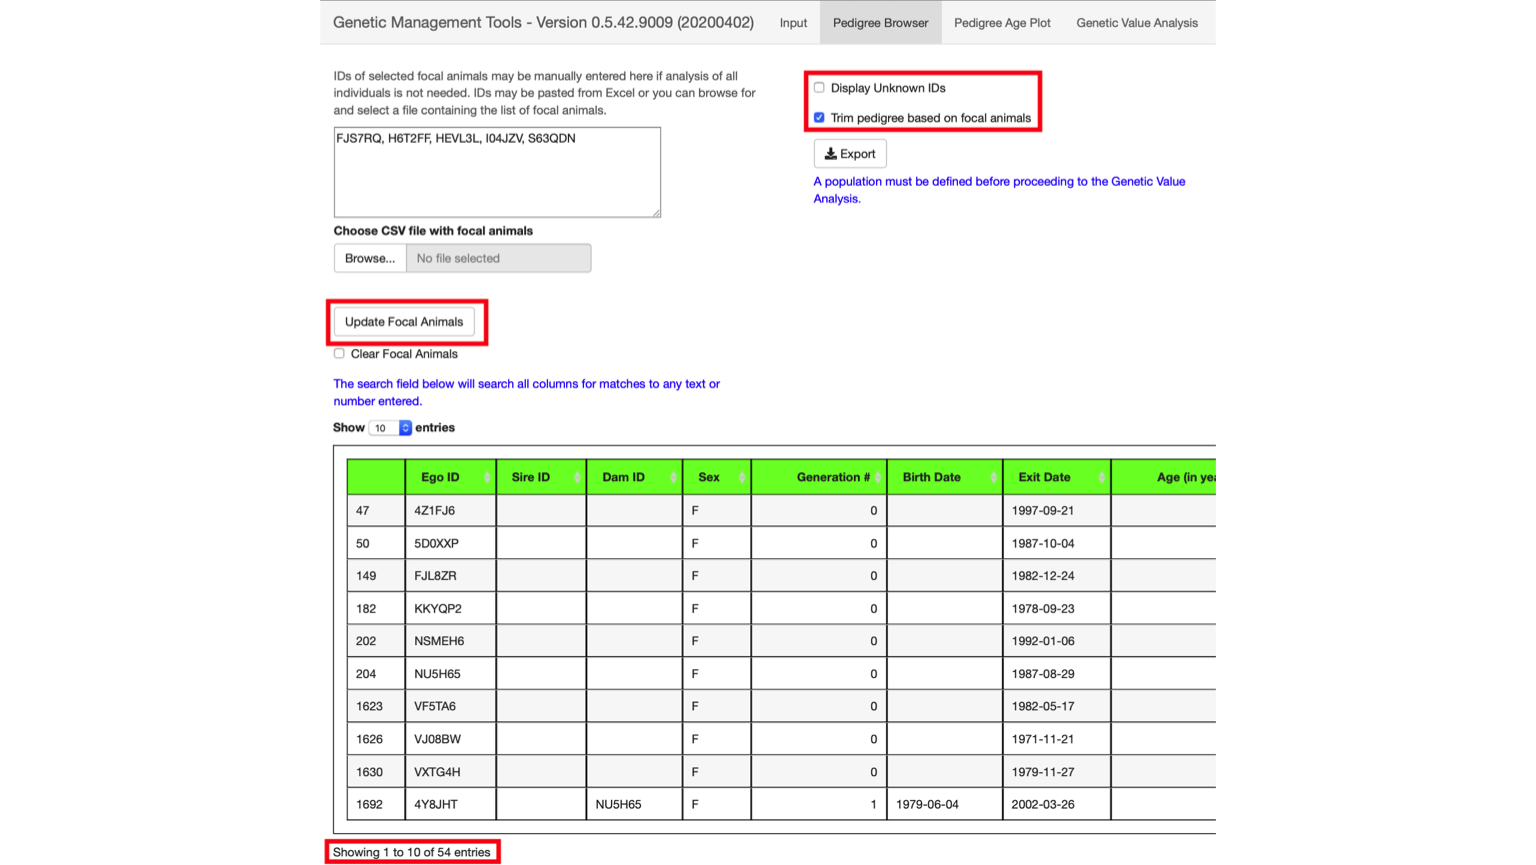
\includegraphics{shiny_app_use_files/figure-latex/pedigree-browser-5-focal-animals-small-1.pdf}

\begin{center}\rule{0.5\linewidth}{\linethickness}\end{center}

Also, you can import a list of focal animals by selecting the
\textbf{Browse} button under \textbf{Choose CSV file with focal
animals}. This file can be constructed by creating a simple text file
with commas between animal IDs or by placing individual animal IDs on
separate lines.

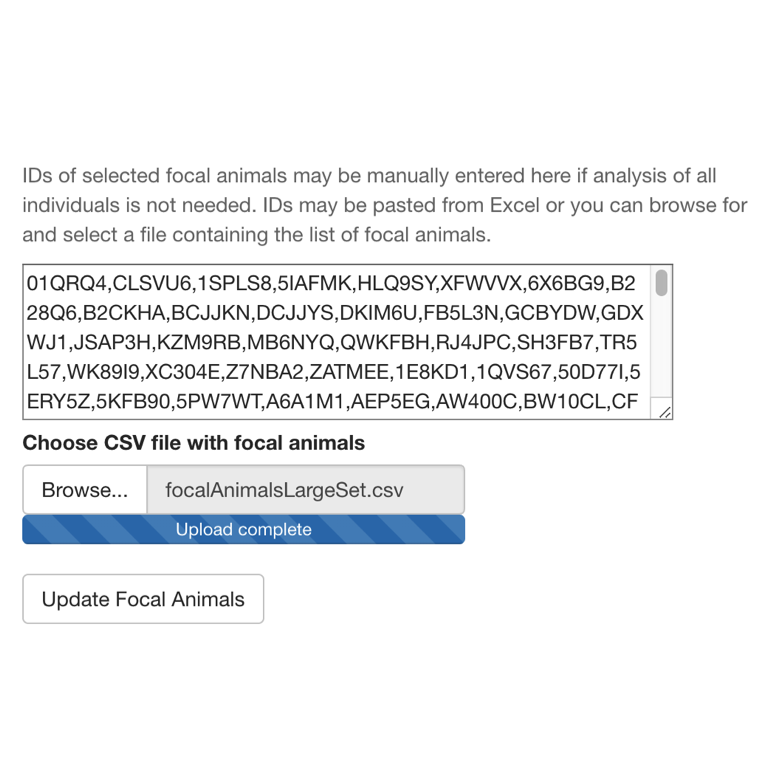
\includegraphics{shiny_app_use_files/figure-latex/selection-large-focal-group-1.pdf}

\begin{center}\rule{0.5\linewidth}{\linethickness}\end{center}

After entering your list of focal animals, you can select to trim the
pedigree so that it will only include relatives of the focal animals you
have selected.

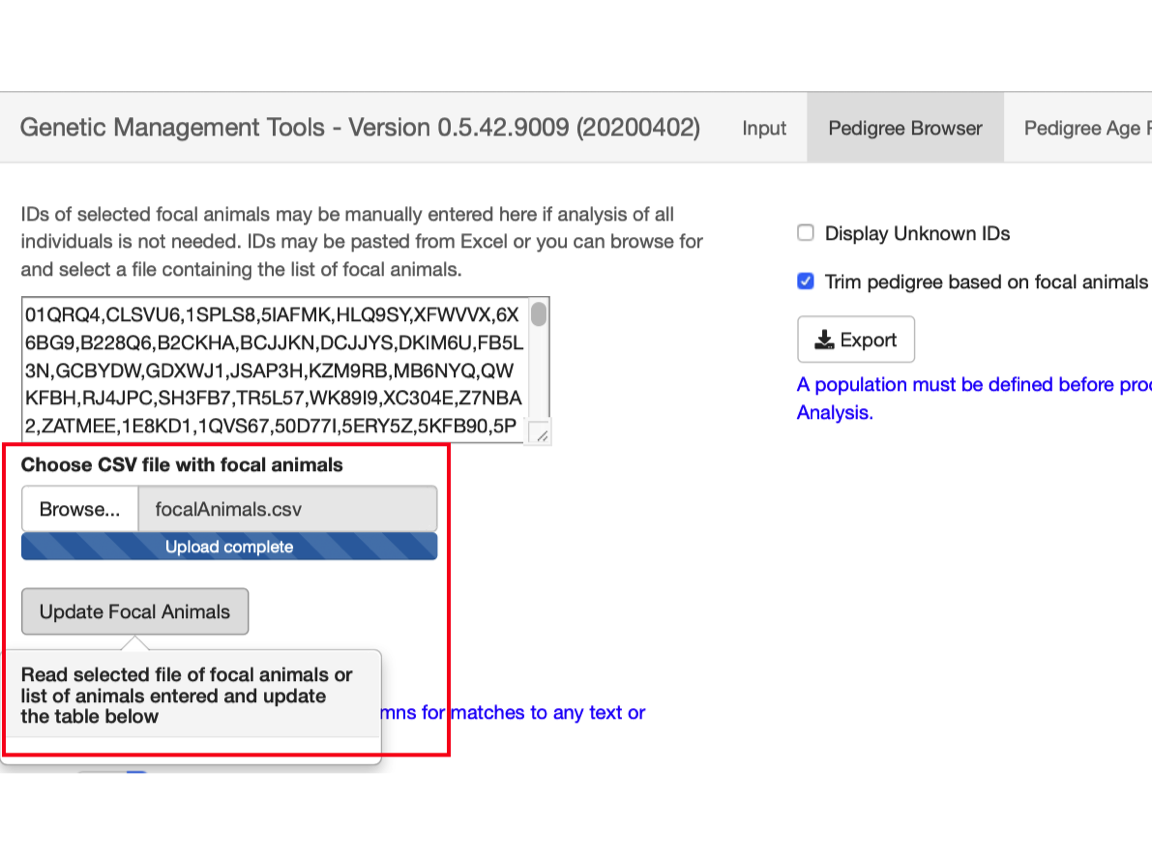
\includegraphics{shiny_app_use_files/figure-latex/select-trim-for-focal-animals-1.pdf}

\begin{center}\rule{0.5\linewidth}{\linethickness}\end{center}

A pedigree trimmed based on focal animals will have only the relatives
of those animals remaining. In this instance there are only a total of
85 focal animals and their relatives.

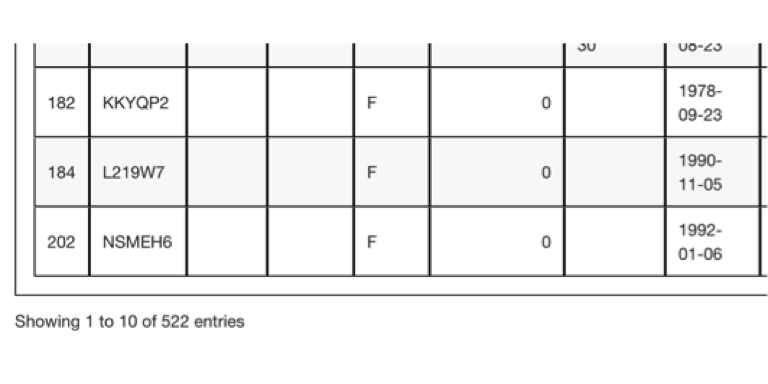
\includegraphics{shiny_app_use_files/figure-latex/trimmed-for-focal-animals-1.pdf}

\begin{center}\rule{0.5\linewidth}{\linethickness}\end{center}

\hypertarget{pedigree-age-pyramid-plot}{%
\subsection{Pedigree Age Pyramid Plot}\label{pedigree-age-pyramid-plot}}

The \textbf{Pedigree Age Plot} tab displays a standard pyramid plot for
the pedigree as selected in the \textbf{Pedigree Browser} tab. This is
showing 332 living animals from the entire example pedigree.

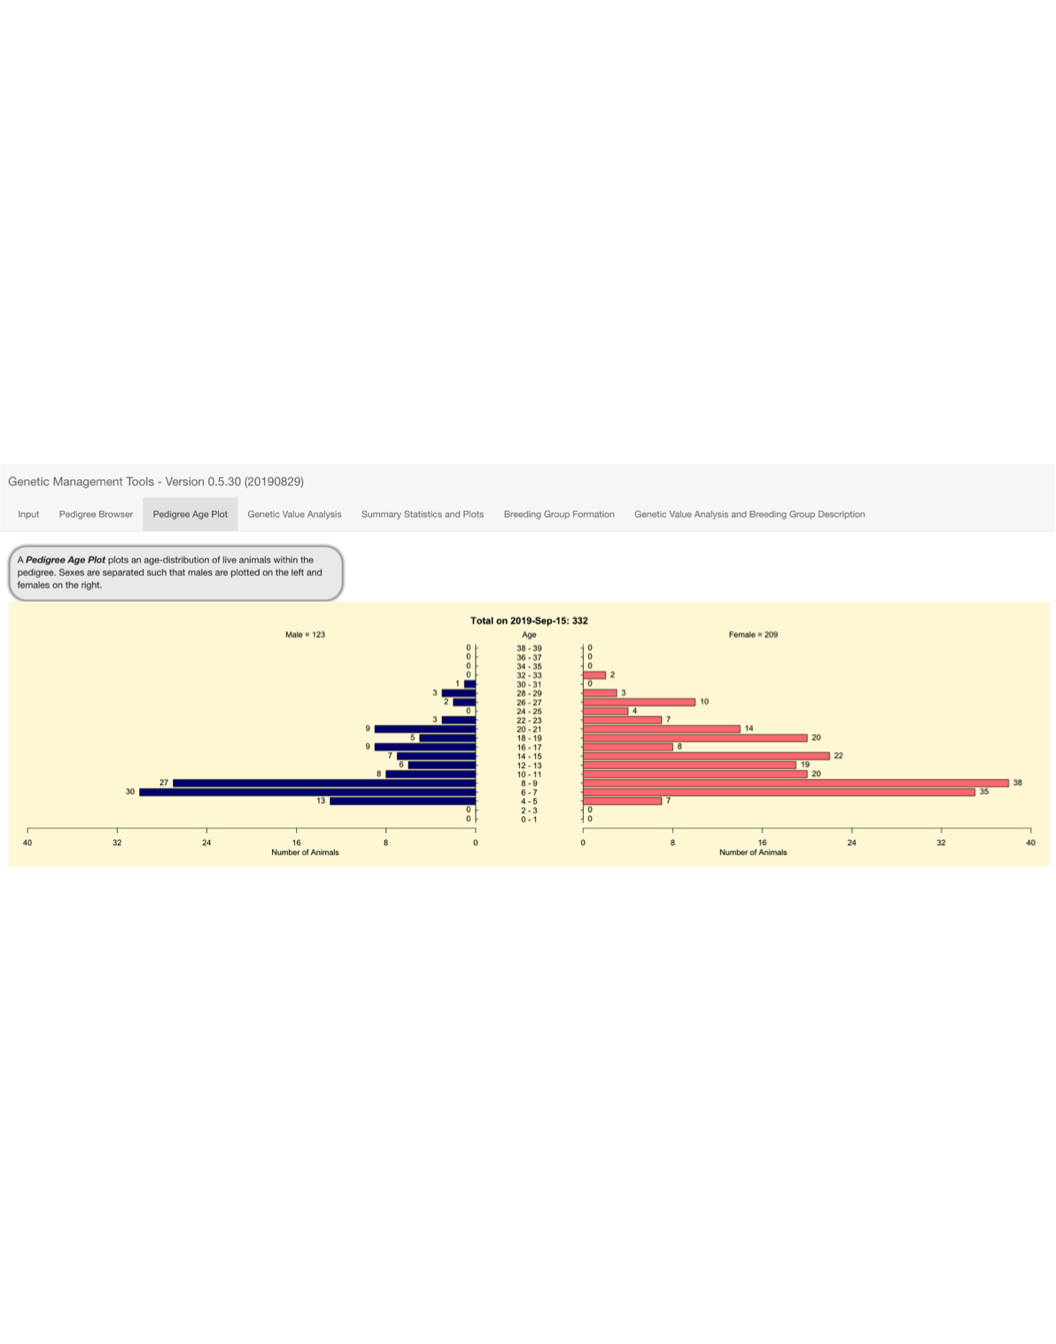
\includegraphics{shiny_app_use_files/figure-latex/age-plot-1.pdf}

\begin{center}\rule{0.5\linewidth}{\linethickness}\end{center}

\hypertarget{genetic-value-analysis}{%
\subsection{Genetic Value Analysis}\label{genetic-value-analysis}}

Selecting the \textbf{Genetic Value Analysis} tab and the \textbf{Begin
Analysis} button will begin the gene dropping process, which you can
monitor with the progress meter in the lower right corner of the
display.

We are not aware of a systematic study of pedigree structure with this
algorithm and have not performed extensive studies with pedigrees of
various structures, but 1000 iterations has seemed to provide
reproducible results.

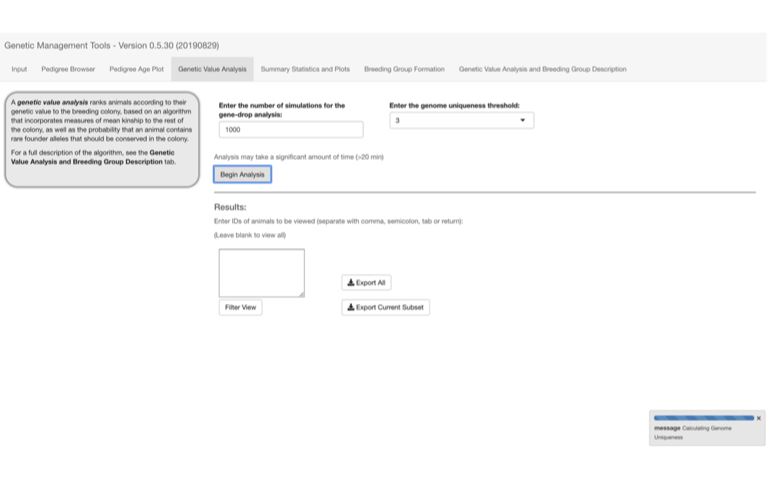
\includegraphics{shiny_app_use_files/figure-latex/gva-calculating-1.pdf}

\begin{center}\rule{0.5\linewidth}{\linethickness}\end{center}

As soon as the calculations are completed, a table showing the results
of the analysis is displayed in 10 record increments. The calculations
for 1000 iterations of the gene dropping algorithm took 1 minute 38
seconds with the example pedigree of 3,691 animals using a MacBook Pro
(Mid 2014), 2.8 GHz Intel Core i7 with 16 GB of 1600 MHz DDR3 memory.

Again you can select how many rows to display at once by changing the
values in the \textbf{Show entries} selection tool.

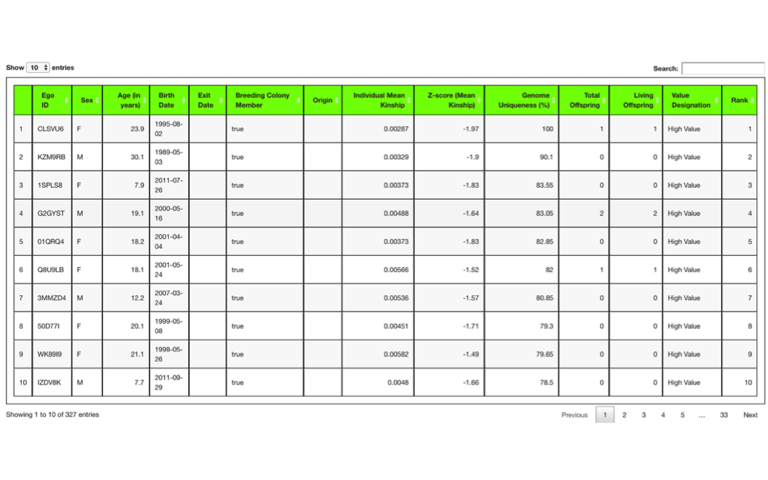
\includegraphics{shiny_app_use_files/figure-latex/gva-first-high-value-1.pdf}

\begin{center}\rule{0.5\linewidth}{\linethickness}\end{center}

Searching down the table of results in the \textbf{Value Designation}
column you can see starting at row 268 the values change from \emph{High
Value} to \emph{Low Value}. Though not shown here, the value of
\emph{Undetermined} in the \textbf{Value Designation} column means the
animal did not have parentage information.

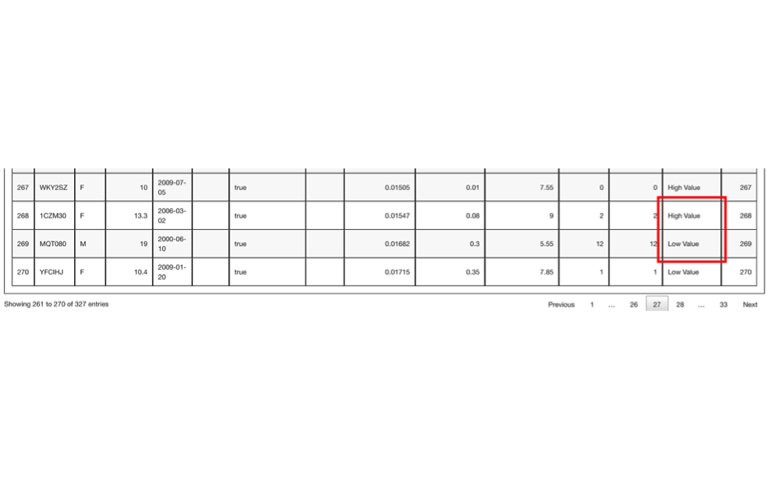
\includegraphics{shiny_app_use_files/figure-latex/gva-high-and-low-value-1.pdf}

\begin{center}\rule{0.5\linewidth}{\linethickness}\end{center}

\hypertarget{summary-statistics}{%
\subsection{Summary Statistics}\label{summary-statistics}}

The \textbf{Summary Statistics and Plots} tab used results from the
\textbf{Genetic Value Analysis} tab.

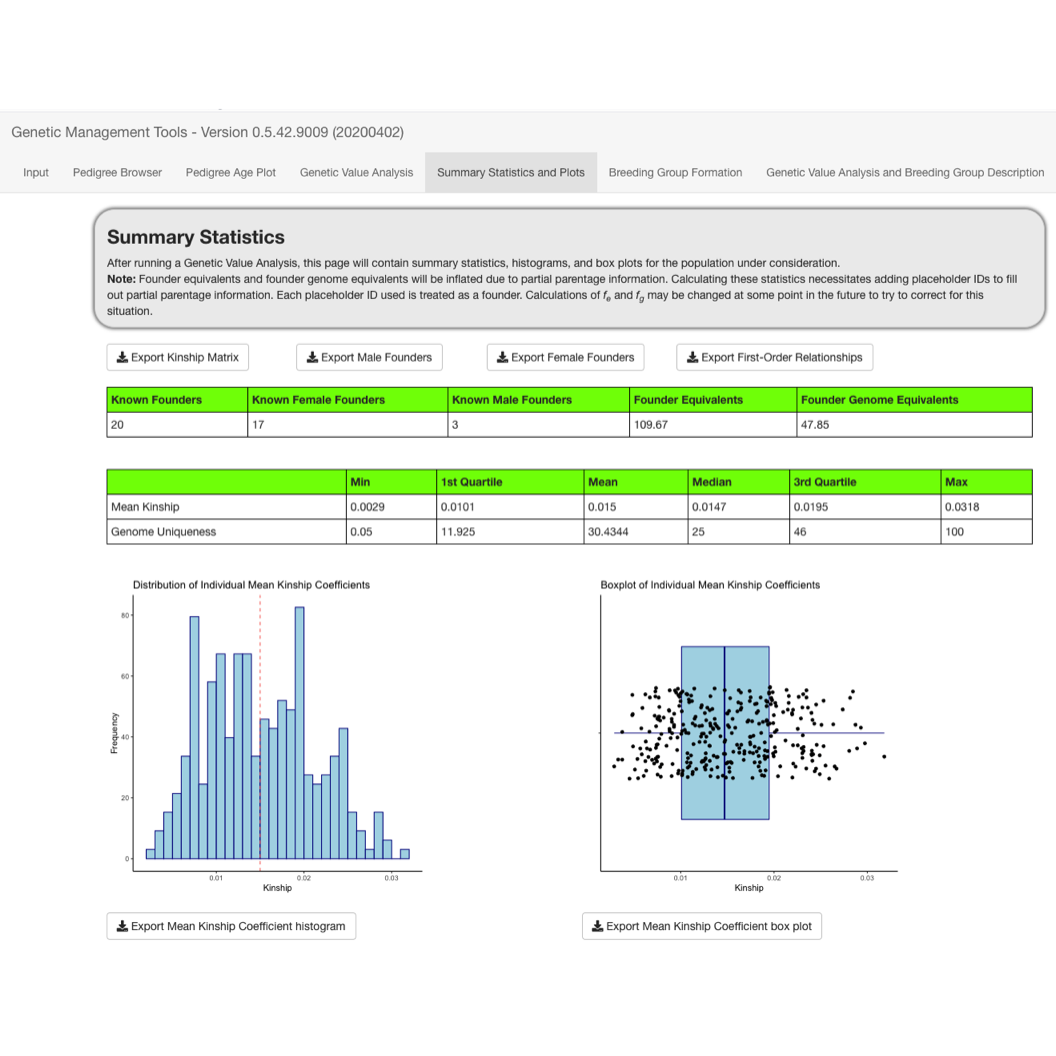
\includegraphics{shiny_app_use_files/figure-latex/ss-first-view-1.pdf}

\begin{center}\rule{0.5\linewidth}{\linethickness}\end{center}

The \textbf{Export Kinship Matrix} button creates a CSV file that has a
row and column for each individual in the genetic analysis plus a first
row and first column each containing the IDs.

The first few rows of such a file are shown below.

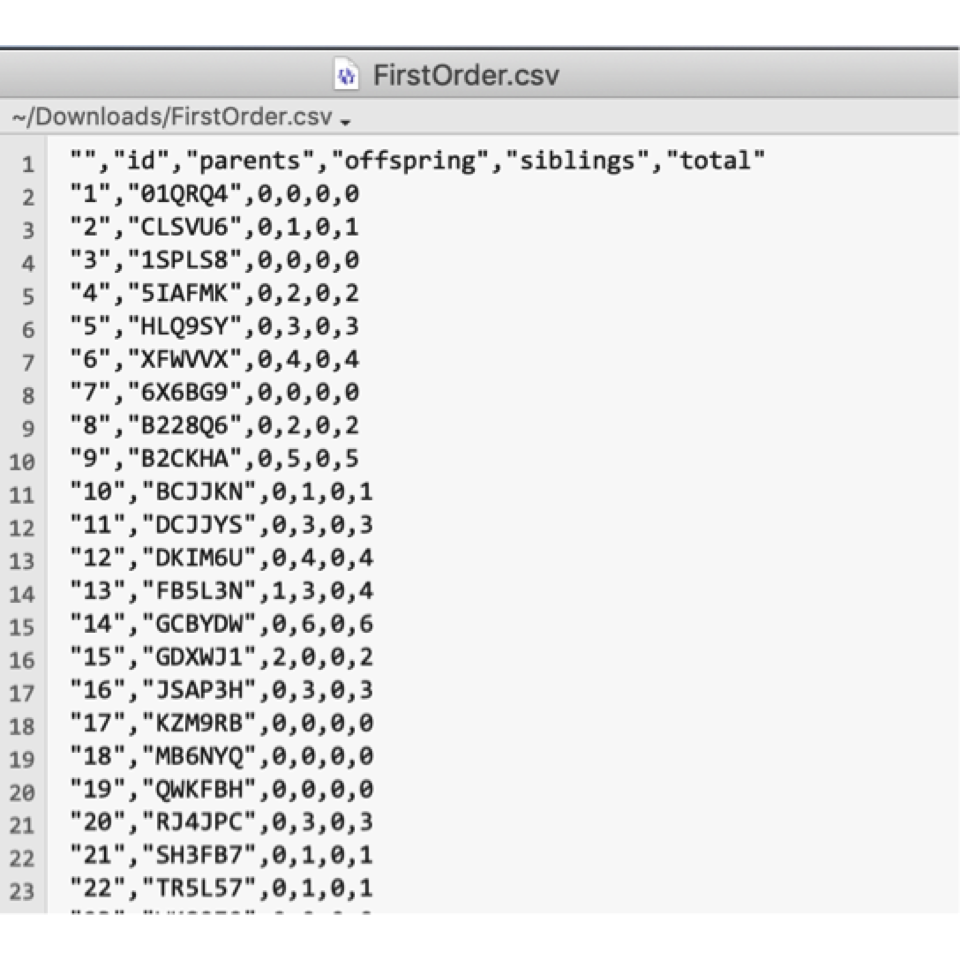
\includegraphics{shiny_app_use_files/figure-latex/first-order-relationships-1.pdf}

\begin{center}\rule{0.5\linewidth}{\linethickness}\end{center}

The \textbf{First-Order Relationships} button creates a CSV file that
has the following columns defined: an unnamed column for row number,
\emph{id}, \emph{parents}, \emph{offspring}, \emph{siblings}, and
\emph{total}. The first few rows of such a file are shown below.

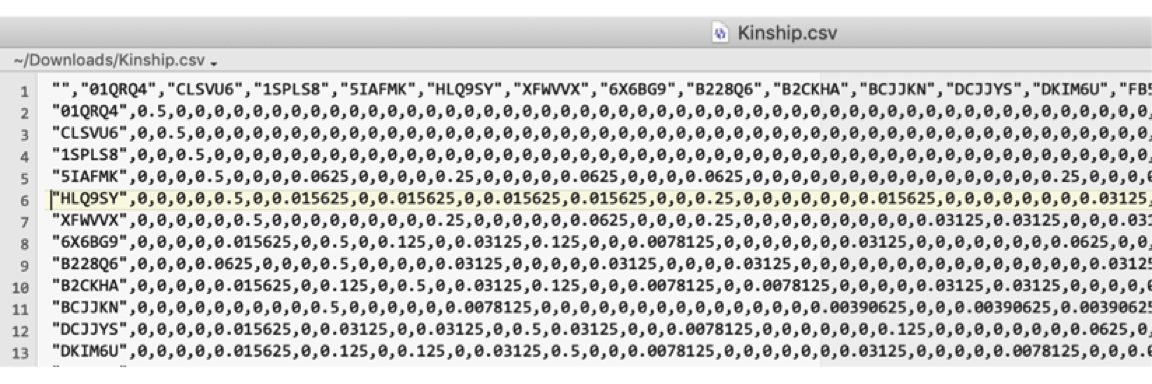
\includegraphics{shiny_app_use_files/figure-latex/ss-kinship-matrix-1.pdf}

\begin{center}\rule{0.5\linewidth}{\linethickness}\end{center}

The six plots provide histograms and boxplots for the kinship
coefficients, the Z-scores of the kinship coefficients, and the genome
uniqueness scores.

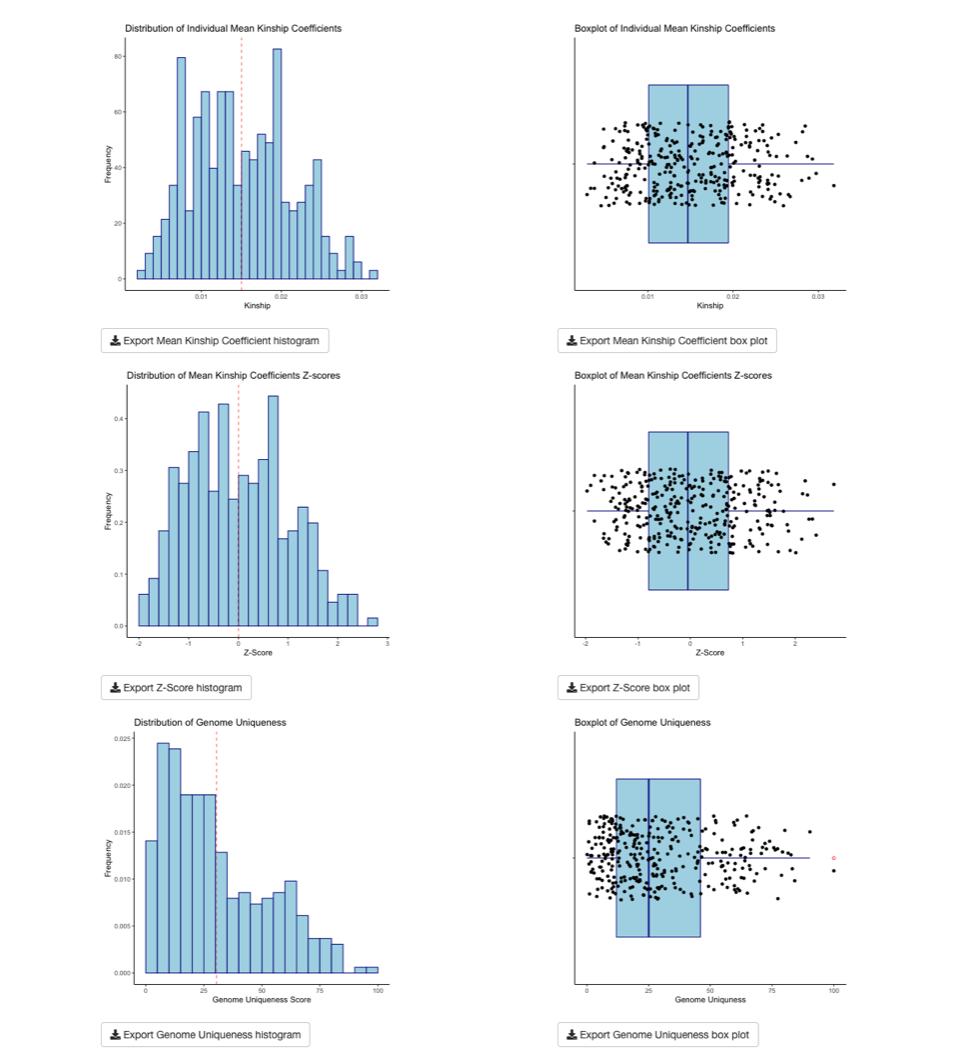
\includegraphics{shiny_app_use_files/figure-latex/ss-trimmed-all-plots-1.pdf}

\begin{center}\rule{0.5\linewidth}{\linethickness}\end{center}

\hypertarget{breeding-group-formation}{%
\subsection{Breeding Group Formation}\label{breeding-group-formation}}

Selecting the \textbf{Breeding Group Formation} tab brings forward the
screen shown below. In this screen you can form breeding groups using
one of three ways based on your source of animals selected under
\textbf{Choose one group formation workflow:}.

Further you must specify how you want to construct the breeding groups
with regard to the groups' sex ratios. The third of the three options
(\emph{User specified sex ratio of breeders}) causes the appearance of
the field where you can fill in the sex ratio (F/M) that you want to
have in the formed breeding groups. The sex ratio algorithm will form a
group as nearly to the selected ratio as possible given the size of the
group. Limits in the availability of either sex will restrict the size
of the groups formed.

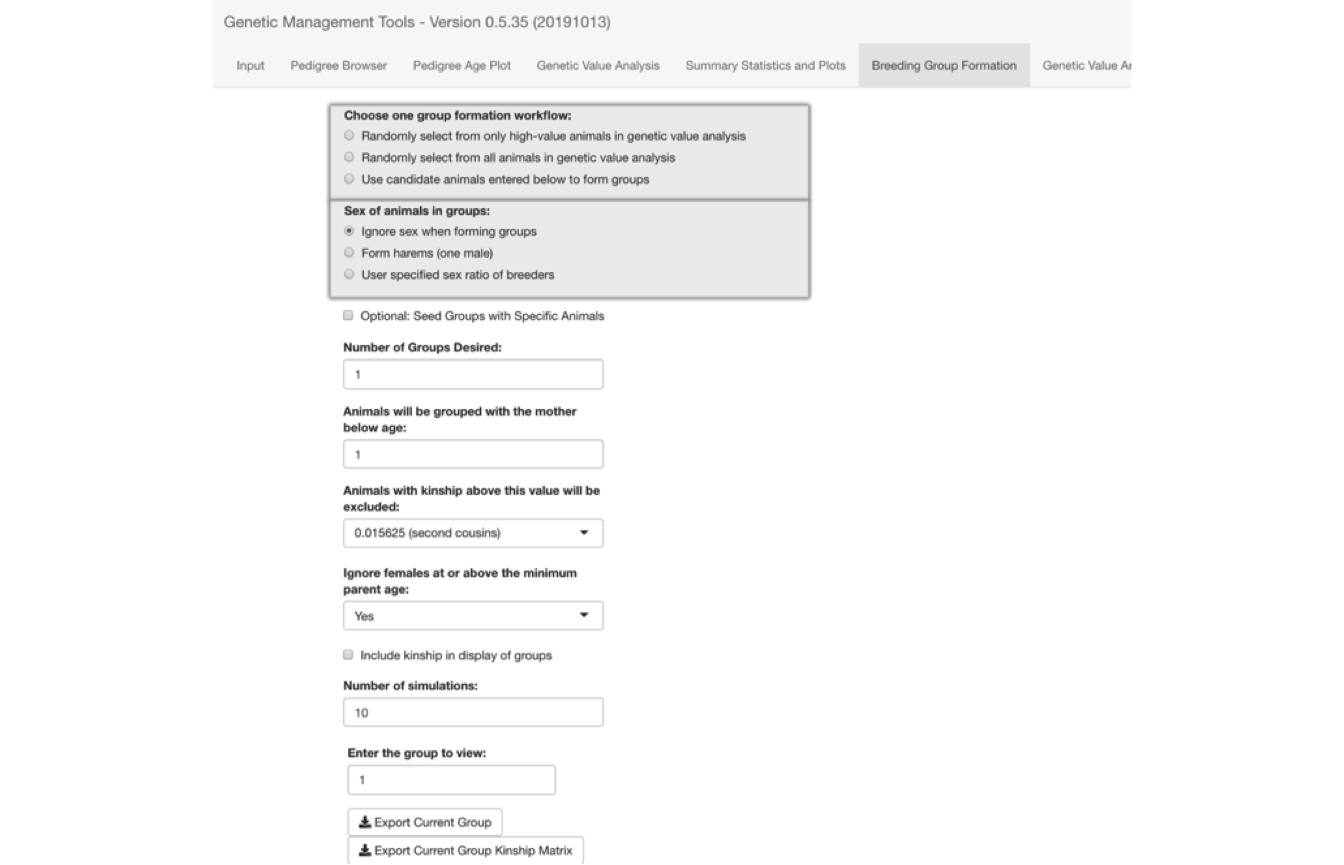
\includegraphics{shiny_app_use_files/figure-latex/breeding-group-first-view-1.pdf}

\begin{center}\rule{0.5\linewidth}{\linethickness}\end{center}

The \textbf{Make Groups} button appears once you select the source of
animals you are going to use. However, you probably will be making
additional selections using other controls on the screen.

The most common source of animals will be the high-value animals found
by the genetic analysis.

You can either type in the number of groups that you want to form or
select the number of groups using the arrows on the right edge of the
\textbf{Number of Groups Desired} field, which is outlined in blue in
the image below.

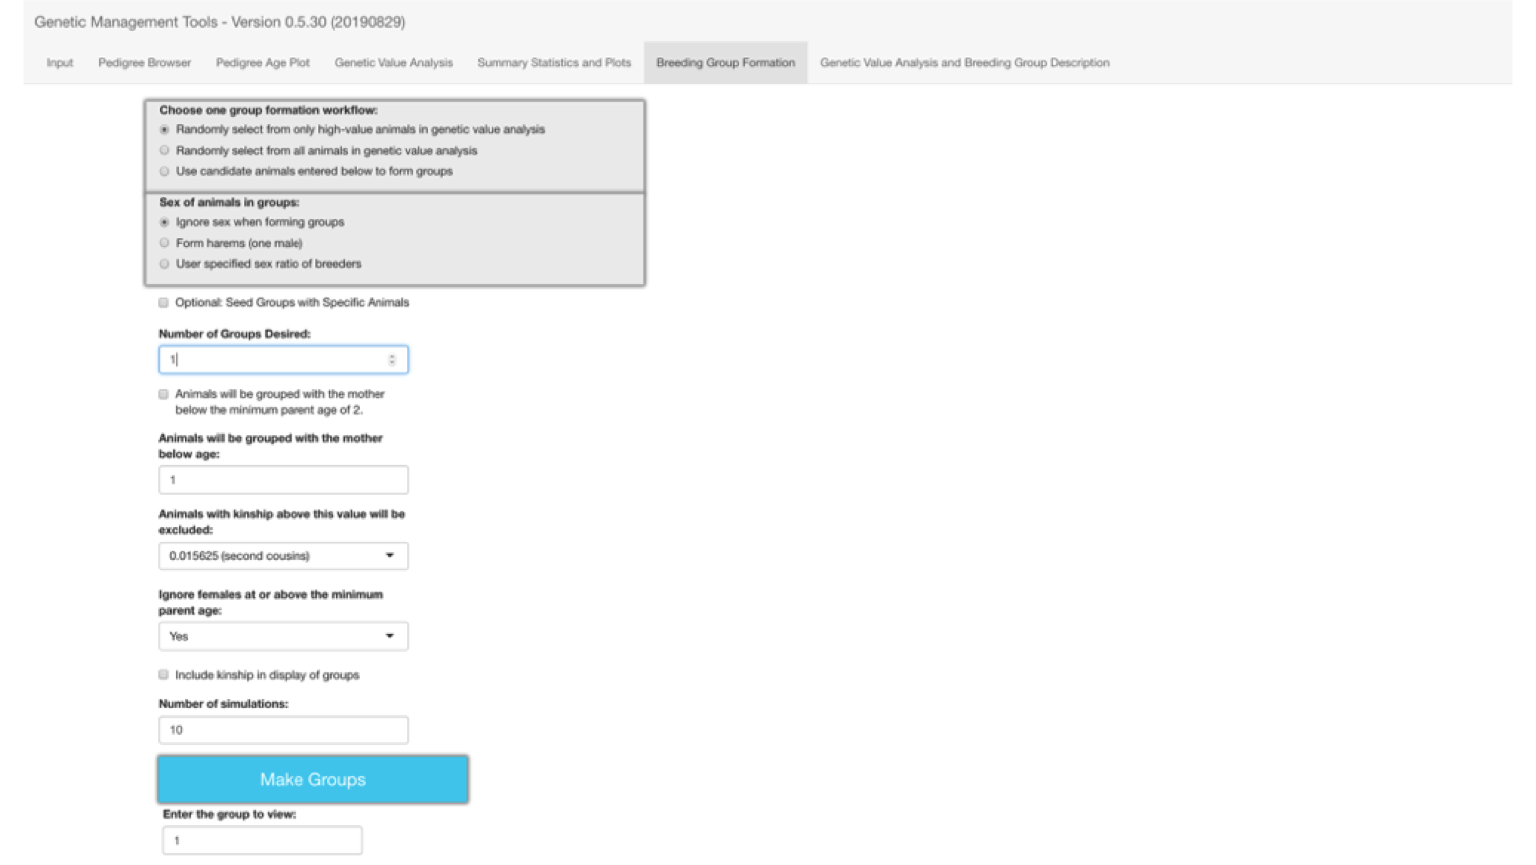
\includegraphics{shiny_app_use_files/figure-latex/breeding-group-1-1.pdf}

\begin{center}\rule{0.5\linewidth}{\linethickness}\end{center}

There are often behavioral constraints, such as preexisting social
groups, that dictate the need to have some animals maintained together.
This need is readily accommodated by pre-seeding groups with those
social groups. You may select the \textbf{Optional: Seed Groups with
Specific Animals} field if you decide to place some animals together
within the groups because you know them to be compatible with each
other.

This has been done in the example below using six groups with differing
numbers of seed animals. Note the selection of having animals below the
minimum parent age of two being grouped with their mother.

\begin{center}\rule{0.5\linewidth}{\linethickness}\end{center}

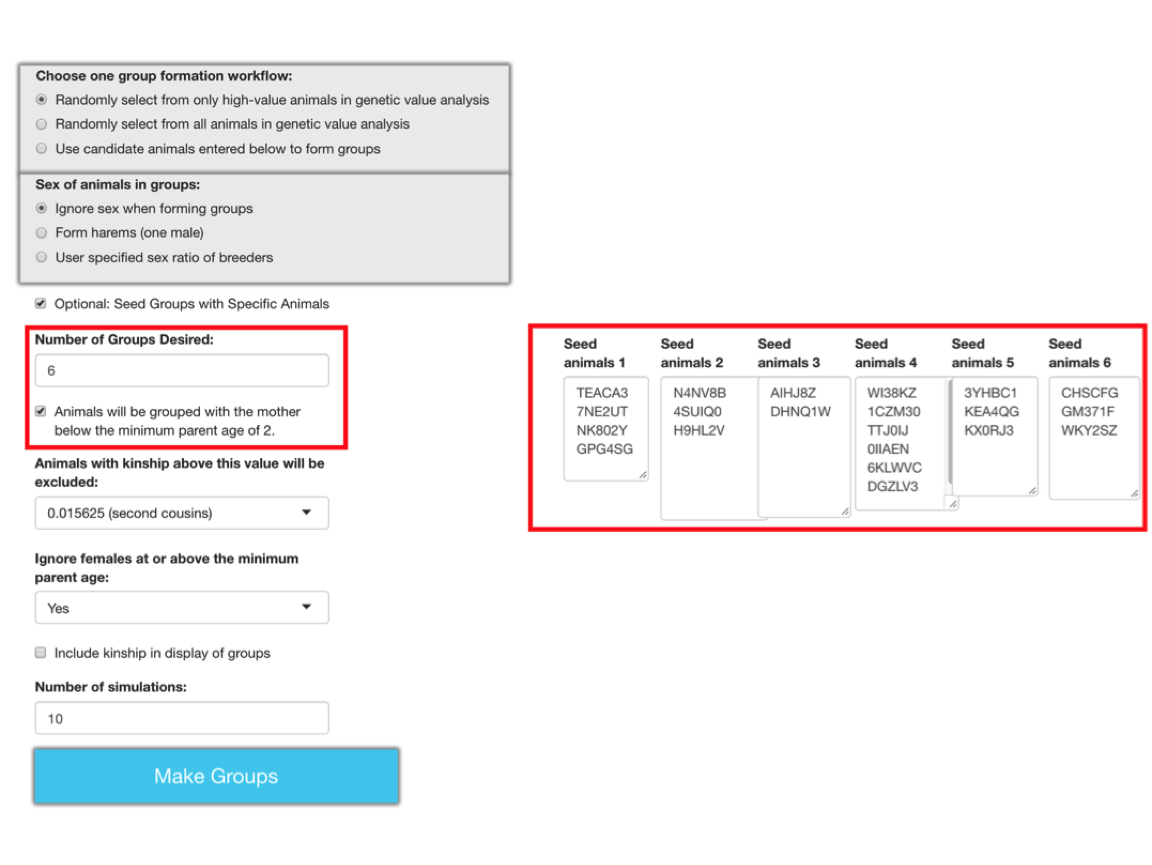
\includegraphics{shiny_app_use_files/figure-latex/breeding-group-6-infants-with-dam-1.pdf}

\begin{center}\rule{0.5\linewidth}{\linethickness}\end{center}

Each group has all of the seed animals that were assigned to it plus
additional animals that could be added while satisfying the requirements
imposed by the selected settings. I have indicated the seed animals for
the first group with red rectangles.

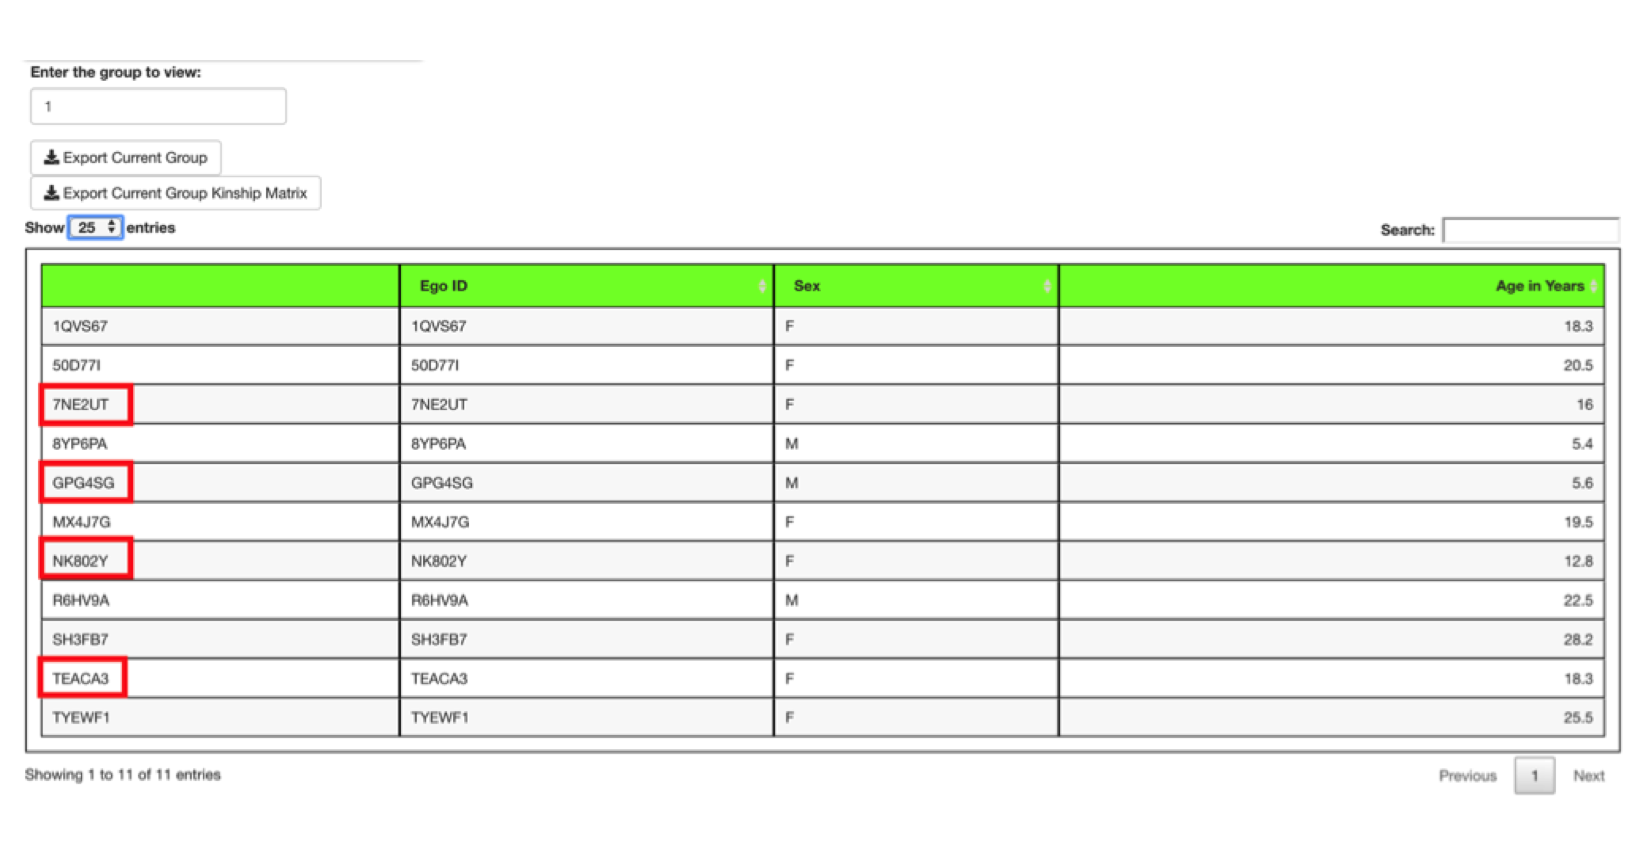
\includegraphics{shiny_app_use_files/figure-latex/breeding-group-first-group-no-kinship-seeds-indicated-1.pdf}

\begin{center}\rule{0.5\linewidth}{\linethickness}\end{center}

Display of kinship values requires that the \textbf{Include kinship in
display of groups} checkbox be selected prior to group formation.

A group of ten animals was formed in the next run after choosing to
include kinship and selecting the \textbf{Make Groups} button.

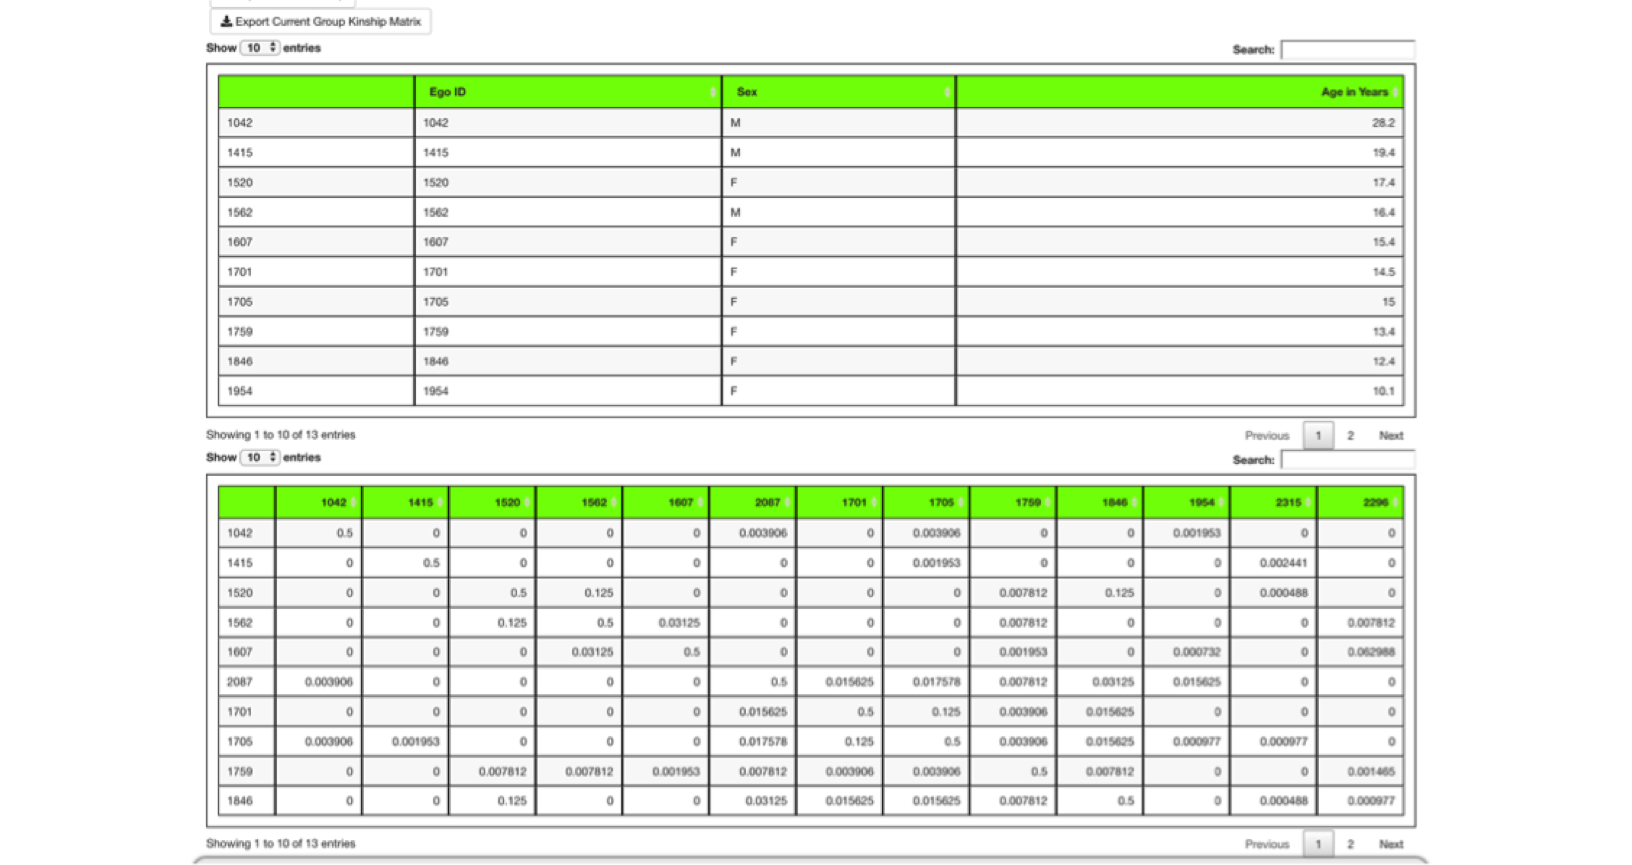
\includegraphics{shiny_app_use_files/figure-latex/breeding-group-6-seed-grps-grp-6-kinship-1.pdf}

\begin{center}\rule{0.5\linewidth}{\linethickness}\end{center}

The option to select a desired sex ratio allows you to select any ratio
desired. However, the ratio obtained is limited by the availability of
animals that meet all criteria you have set.

\end{document}
